\chapter{算例分析}
\label{cha:Example}

\section{算例}

设想一个四节点机组网络有向图如图~\ref{fig:Directed-graph}:

%去除Visio白边:http://www.mamicode.com/info-detail-2181323.html

\begin{figure}[htbp] % use float package if you want it here
    \centering
    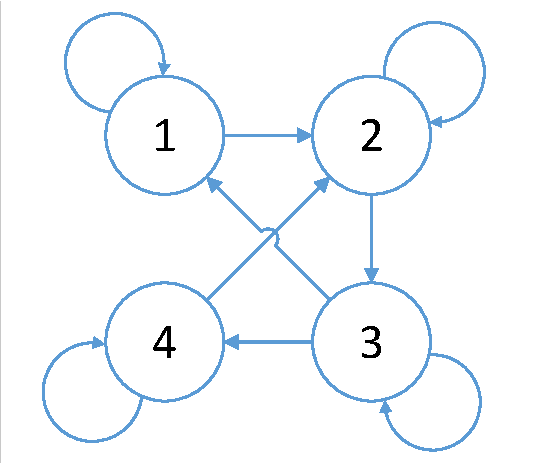
\includegraphics{Directed-graph.pdf}
    \caption{四节点机组网络有向图}
    \label{fig:Directed-graph}
\end{figure}

各节点处机组参数与负荷如表~\ref{tab:example}:

\begin{table}[]
    \centering
%    \resizebox{\textwidth}{!}{%
    \begin{tabular}{@{}ccccc@{}}
    \toprule
    \multicolumn{1}{c}{Node} & $\alpha_{i}(\mathrm{MW})$  & $\beta_{i} \quad\left(\mathrm{MW}^{2} / \mathrm{S}\right)$ & $\gamma_{i}(\mathrm{S})$   & $L_{i}(\mathrm{MW})$    \\ \midrule
    1                        & -1 & 1 & 0.2 & 15.5 \\
    2                        & -2 & 2 & 0.1 & 0    \\
    3                        & -3 & 3 & 0.5 & 15.5 \\
    4                        & -1 & 2 & 0.7 & 0    \\ \bottomrule
    \end{tabular}
%    }缩放表格(字会变得很大)
    \caption{4节点算例机组参数与实时负荷}
    \label{tab:example}
\end{table}

其邻接矩阵为:

\begin{equation}
    A=\left[\begin{array}{cccc}
    {1} & {1} & {0} & {0} \\
    {0} & {1} & {1} & {0} \\
    {1} & {0} & {1} & {1} \\
    {0} & {1} & {0} & {1}
    \end{array}\right]
\end{equation}


\section{普通算法}


简单取平均后得到过渡矩阵为:

\begin{equation}
    Q=\left[\begin{array}{cccc}
    {\frac{1}{2}} & {\frac{1}{2}} & {0} & {0} \\
    {0} & {\frac{1}{2}} & {\frac{1}{2}} & {0} \\
    {\frac{1}{3}} & {0} & {\frac{1}{3}} & {\frac{1}{3}} \\
    {0} & {\frac{1}{2}} & {0} & {\frac{1}{2}}
    \end{array}\right]
\end{equation}

进行迭代:

\section{优化后的算法}

随着迭代各机组的价格曲线如图所示